% ============================================================
% ECON 308 — International Economic Relations
% Lecture 2: Labour Productivity and Comparative Advantage
%            The Ricardian Model  (Chapter 3)
% Fall 2026  |  Muhebullah Karimzada  |  UNBC
% ============================================================
\documentclass[aspectratio=169]{beamer}
\usepackage[utf8]{inputenc}
\usepackage[T1]{fontenc}
\usepackage{lmodern}
\usepackage{textcomp}

%% ── Theme and colours ───────────────────────────────────────
\usetheme{Madrid}
\setbeamertemplate{navigation symbols}{}
\setbeamercovered{transparent}
\setbeamertemplate{itemize items}[circle]
\setbeamertemplate{enumerate items}[default]
\setlength{\parskip}{0.15em}

\definecolor{UNBCDark}    {RGB}{0,74,37}
\definecolor{UNBCGold}    {RGB}{189,155,96}
\definecolor{SoftGray}    {RGB}{244,246,248}
\definecolor{AccentRed}   {RGB}{192,57,43}
\definecolor{AccentBlue}  {RGB}{41,98,255}
\definecolor{AccentTeal}  {RGB}{0,150,136}
\definecolor{AccentOrange}{RGB}{230,126,34}

\setbeamercolor{normal text}         {fg=black,bg=white}
\setbeamercolor{structure}           {fg=UNBCDark}
\setbeamercolor{title}               {fg=white,bg=UNBCDark}
\setbeamercolor{subtitle}            {fg=UNBCGold}
\setbeamercolor{frametitle}          {fg=white,bg=UNBCDark}
\setbeamercolor{block title}         {fg=white,bg=UNBCDark}
\setbeamercolor{block body}          {fg=black,bg=SoftGray}
\setbeamercolor{block title alerted} {fg=white,bg=AccentRed}
\setbeamercolor{block body alerted}  {fg=black,bg=SoftGray}
\setbeamercolor{item}                {fg=UNBCDark}
\setbeamercolor{alerted text}        {fg=AccentRed}
\setbeamercolor{author in head/foot} {fg=white,bg=UNBCDark}
\setbeamercolor{date in head/foot}   {fg=white,bg=UNBCDark}

%% ── Packages ────────────────────────────────────────────────
\usepackage{booktabs,multirow,array,amsmath,amssymb,bm,
            graphicx,adjustbox,tikz,pgfplots,tcolorbox,hyperref}
\tcbuselibrary{skins}
\pgfplotsset{compat=1.18}
\usetikzlibrary{arrows.meta,positioning,calc,shapes.geometric}
\hypersetup{colorlinks=true,linkcolor=UNBCDark}

%% ── Footline ────────────────────────────────────────────────
\setbeamertemplate{headline}{}
\setbeamertemplate{footline}{%
  \leavevmode\hbox{%
  \begin{beamercolorbox}[wd=.78\paperwidth,ht=2.6ex,dp=1.0ex,
                         leftskip=1em]{author in head/foot}%
    \color{white}\textbf{ECON 308}\hspace{0.4em}%
    \textcolor{UNBCGold}{$\vert$}\hspace{0.4em}%
    International Economic Relations%
  \end{beamercolorbox}%
  \begin{beamercolorbox}[wd=.22\paperwidth,ht=2.6ex,dp=1.0ex,
                         rightskip=1em plus 1fil]{date in head/foot}%
    \color{white}\hfill\insertframenumber/\inserttotalframenumber%
  \end{beamercolorbox}}%
}

%% ── Custom tcolorboxes (compact padding) ────────────────────
\newtcolorbox{insight}[1]{%
  colback=UNBCGold!12,colframe=UNBCGold!70!black,
  title={\small\bfseries #1},
  left=1mm,right=1mm,top=0.4mm,bottom=0.4mm,
  boxrule=0.5pt,arc=2mm}

\newtcolorbox{canadex}[1][Canadian Example]{%
  colback=AccentTeal!9,colframe=AccentTeal,
  title={\small\bfseries #1},
  left=1mm,right=1mm,top=0.4mm,bottom=0.4mm,
  boxrule=0.5pt,arc=2mm}

\newtcolorbox{discuss}{%
  colback=AccentBlue!8,colframe=AccentBlue,
  title={\small\bfseries Discussion},
  left=1mm,right=1mm,top=0.4mm,bottom=0.4mm,
  boxrule=0.5pt,arc=2mm}

\newtcolorbox{worked}{%
  colback=AccentOrange!8,colframe=AccentOrange,
  title={\small\bfseries Worked Example},
  left=1mm,right=1mm,top=0.4mm,bottom=0.4mm,
  boxrule=0.5pt,arc=2mm}

\newtcolorbox{varbox}{%
  colback=SoftGray,colframe=UNBCDark!40,
  left=1mm,right=1mm,top=0.4mm,bottom=0.4mm,
  boxrule=0.4pt,arc=2mm}

%% ── Metadata ────────────────────────────────────────────────
\title{\textbf{Labour Productivity \& Comparative Advantage}}
\subtitle{{\large ECON 308\enspace International Economic
  Relations\enspace\textcolor{UNBCGold}{$|$}\enspace
  Chapter~3: The Ricardian Model}}
\author{Muhebullah Karimzada}
\institute{School of Economics\\
           University of Northern British Columbia}
\date{Fall 2026}

% ============================================================
\begin{document}
% ============================================================

%% ─────────────────────────────────────────────────────────────
%% 1. TITLE
%% ─────────────────────────────────────────────────────────────
\begin{frame}[plain]
\titlepage
\end{frame}

%% ─────────────────────────────────────────────────────────────
%% 2. OPENING PUZZLE
%% ─────────────────────────────────────────────────────────────
\begin{frame}{Opening Puzzle: How Can Bangladesh Compete?}
\begin{columns}[T]
\begin{column}{0.57\textwidth}
\begin{itemize}
  \item Bangladesh has \textbf{lower labour productivity
        than Canada in every industry}: garments,
        electronics, agriculture, steel.
  \item Yet Bangladesh is a \textbf{top-five global
        garment exporter} (\$34 billion, 2019).
  \item Canada imports Bangladeshi clothing by the
        billions despite being more productive at
        \emph{everything}.
  \item \textbf{Why does trade happen?}
\end{itemize}
\vspace{0.4em}
\begin{insight}{David Ricardo's Answer (1817)}
\small Absolute productivity does \emph{not} determine
trade.  A country exports where its \textbf{opportunity
cost is lowest}.  This is
\textbf{comparative advantage}.
\end{insight}
\end{column}
\begin{column}{0.40\textwidth}
\begin{center}
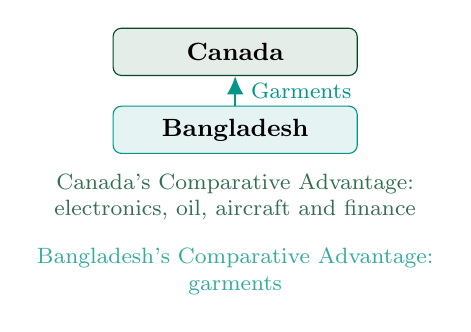
\begin{tikzpicture}[scale=0.90,
  box/.style={draw,rounded corners=3pt,font=\small\bfseries,
              minimum width=3.1cm,minimum height=0.6cm,
              align=center}]
  \node[box,draw=UNBCDark,fill=UNBCDark!10] (CA) at (0,3.3)
        {Canada};
  \node[box,draw=AccentTeal,fill=AccentTeal!10] (BD) at (0,2.2)
        {Bangladesh};
  \draw[-{Latex[width=6pt]},AccentTeal,thick]
        (BD.north)--(CA.south)
        node[midway,right=2pt,font=\footnotesize]
        {Garments};
  \node[font=\footnotesize,align=center,text=UNBCDark!80]
        at (0,1.1) {Canada's Comparative Advantage:\\ electronics, oil,
        aircraft and finance\\};
  \node[font=\footnotesize,align=center,text=AccentTeal!80]
        at (0,0.2) {Bangladesh's Comparative Advantage:\\ garments};
\end{tikzpicture}
\end{center}
\end{column}
\end{columns}
\end{frame}

%% ─────────────────────────────────────────────────────────────
%% 3. COURSE POSITION
%% ─────────────────────────────────────────────────────────────
\begin{frame}{Where We Are in the Course}
\begin{columns}[T]
\begin{column}{0.55\textwidth}
\textbf{Chapter 3 is the foundation of all trade theory:}
\begin{itemize}\small
  \item \textbf{Ch.~2} (Lecture~1): \emph{What} are the
        facts?  Who trades with whom?  The gravity model.
  \item \textbf{Ch.~3} (today): \emph{Why} trade?
        Comparative advantage determines the pattern of
        trade.
  \item \textbf{Ch.~4}: Short run -- capital is
        sector-specific.  Trade creates winners
        \emph{and} losers within a country.
  \item \textbf{Ch.~5}: Long run -- the Heckscher-Ohlin
        model.  Factor endowments determine trade.
\end{itemize}
\vspace{0.3em}
\begin{varbox}
\footnotesize\textbf{Why one factor?}
The Ricardian model uses \emph{labour only} to isolate
technology as the source of comparative advantage.  Capital and land are
added in Chapters~4--5.
\end{varbox}
\end{column}
\begin{column}{0.42\textwidth}
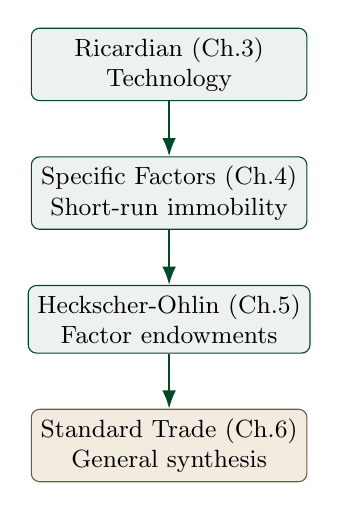
\begin{tikzpicture}[node distance=0.7cm,
  box/.style={draw=UNBCDark,fill=UNBCDark!7,rounded corners=3pt,
              minimum width=3.5cm,minimum height=0.65cm,
              align=center,font=\small}]
  \node[box] (R) {Ricardian (Ch.3)\\Technology};
  \node[box,below=of R] (S)
        {Specific Factors (Ch.4)\\Short-run immobility};
  \node[box,below=of S] (H)
        {Heckscher-Ohlin (Ch.5)\\Factor endowments};
  \node[box,below=of H,fill=UNBCGold!20,draw=UNBCGold!60!black]
        (ST) {Standard Trade (Ch.6)\\General synthesis};
  \draw[-{Latex},UNBCDark,thick] (R)--(S);
  \draw[-{Latex},UNBCDark,thick] (S)--(H);
  \draw[-{Latex},UNBCDark,thick] (H)--(ST);
\end{tikzpicture}
\end{column}
\end{columns}
\end{frame}

%% ─────────────────────────────────────────────────────────────
%% 4. LEARNING OBJECTIVES
%% ─────────────────────────────────────────────────────────────
\begin{frame}{Learning Objectives}
After this lecture you will be able to:
\begin{enumerate}\small
  \item Distinguish \textbf{absolute advantage} from
        \textbf{comparative advantage} (CA) and explain why
        only CA determines trade.
  \item Compute \textbf{opportunity costs} from unit
        labour requirements (ULRs).
  \item Derive a country's linear \textbf{production
        possibility frontier} and autarky relative price.
  \item Explain the \textbf{pattern of specialisation}
        and the valid range of the terms of trade.
  \item Show that \textbf{both countries gain} by
        consuming beyond their PPFs.
  \item Explain why \textbf{wages reflect productivity}
        and refute the pauper-labour fallacy.


\end{enumerate}
\begin{block}{}
\small Krugman, Obstfeld \& Melitz,
\textit{International Economics}, 12th ed., Chapter~3.
\end{block}
\end{frame}

%% ═══════════════════════════════════════════════════════════
%%  PART 1 — COMPARATIVE ADVANTAGE
%% ═══════════════════════════════════════════════════════════

%% ─────────────────────────────────────────────────────────────
%% 5. ABSOLUTE vs COMPARATIVE
%% ─────────────────────────────────────────────────────────────
\begin{frame}[shrink=12]{Absolute vs.\ Comparative Advantage}
\begin{columns}[T]
\begin{column}{0.50\textwidth}
\begin{block}{Absolute Advantage}
\small Country A needs \emph{fewer labour hours} per unit:
$a_{LX} < a_{LX}^{*}$.  A is simply more efficient.
\end{block}
\vspace{0.3em}
\begin{block}{Comparative Advantage}
\small Country A's \emph{opportunity cost} of $X$ is lower:
\[\frac{a_{LX}}{a_{LY}} < \frac{a_{LX}^{*}}{a_{LY}^{*}}\]
A gives up less of $Y$ to produce one extra unit of $X$.
\end{block}
\vspace{0.3em}
\begin{varbox}
\footnotesize\textbf{Ricardo's insight:} Even if A is better
at \emph{everything}, trade is mutually beneficial as long as
opportunity costs differ.  What you \emph{give up} matters.
\end{varbox}
\end{column}
\begin{column}{0.47\textwidth}
\begin{varbox}
\small\textbf{The key test for CA}\\[0.2em]
Compare the \emph{ratio} $a_{LX}/a_{LY}$ across countries,
not the levels.  The country with the \emph{lower ratio}
has CA in $X$.\\[0.3em]
\textbf{Cloth/Wine example:}\\[0.1em]
\begin{tabular}{lcc}
& Home & Foreign\\\midrule
$a_{LC}/a_{LW}$ & $1/2$ & $6/3=2$
\end{tabular}\\[0.2em]
$1/2 < 2$ $\Rightarrow$ Home: CA in \textbf{cloth}.\\
Reciprocal: Foreign: CA in \textbf{wine}.
\end{varbox}
\vspace{0.3em}

\end{column}
\end{columns}
\end{frame}

%% ─────────────────────────────────────────────────────────────
%% 6. OPPORTUNITY COST STEP BY STEP
%% ─────────────────────────────────────────────────────────────
\begin{frame}{Opportunity Cost: The Step-by-Step Logic}
\begin{columns}[T]
\begin{column}{0.52\textwidth}
\textbf{OC of cloth for Home ($a_{LC}=1$, $a_{LW}=2$):}
\begin{enumerate}\small
  \item 1 cloth requires $a_{LC} = 1$ labour hour.
  \item Those hours could produce $a_{LC}/a_{LW}
        = 1/2$ wine.
  \item \textbf{OC of 1 cloth $= 1/2$ wine.}
\end{enumerate}
\vspace{0.4em}
\textbf{Autarky price under perfect competition:}
\[\frac{P_C}{P_W} = \frac{w\,a_{LC}}{w\,a_{LW}}
  = \frac{a_{LC}}{a_{LW}} = \text{opportunity cost}\]
\vspace{0.1em}
\textbf{CA condition (Home has CA in cloth):}
\[
\underbrace{\frac{a_{LC}}{a_{LW}}}_{\text{Home OC}}
\;<\;
\underbrace{\frac{a_{LC}^{*}}{a_{LW}^{*}}}_{\text{Foreign OC}}
\]
\end{column}
\begin{column}{0.45\textwidth}
\begin{varbox}
\footnotesize\textbf{OC of wine for Home:}\\
1 wine $=a_{LW}=2$ hours, could yield $a_{LW}/a_{LC}=2$
cloth.  OC of wine $= 2$ cloth.\\[0.3em]
\textbf{OCs are reciprocals:}
$\;\text{OC}_C \times \text{OC}_W = 1$.\\[0.3em]
If Home has CA in cloth, Foreign \emph{must} have CA in
wine.
\end{varbox}
\vspace{0.4em}
\begin{insight}{Autarky Price $=$ OC}
\footnotesize Under perfect competition, relative prices
equal relative unit labour costs~-- which equal
opportunity costs.\\[0.2em]
Technology maps directly to prices:\\
$P_C/P_W = a_{LC}/a_{LW}$ in autarky.
\end{insight}
\end{column}
\end{columns}
\end{frame}

%% ─────────────────────────────────────────────────────────────
%% 7. NUMERICAL EXAMPLE
%% ─────────────────────────────────────────────────────────────
\begin{frame}{Numerical Example: Home and Foreign}
\begin{center}
\begin{adjustbox}{max width=0.92\textwidth}
\begin{tabular}{lccccl}
\toprule
\textbf{Country}&$a_{LC}$&$a_{LW}$&
\textbf{OC of cloth}&\textbf{OC of wine}&\textbf{CA}\\
\midrule
Home   & 1 hr & 2 hrs & $\tfrac{1}{2}$ wine &
         2 cloth & \textbf{Cloth}\\
Foreign& 6 hrs& 3 hrs & 2 wine &
         $\tfrac{1}{2}$ cloth & \textbf{Wine}\\
\bottomrule
\end{tabular}
\end{adjustbox}
\end{center}
\vspace{0.2em}
\begin{columns}[T]
\begin{column}{0.50\textwidth}
\textbf{Absolute advantage:}
\begin{itemize}\small
  \item Cloth: Home (1 hr) vs.\ Foreign (6 hrs)
        $\Rightarrow$ Home $6\times$ faster.
  \item Wine: Home (2 hrs) vs.\ Foreign (3 hrs)
        $\Rightarrow$ Home $1.5\times$ faster.
  \item \textbf{Home absolutely better at both goods.}
\end{itemize}
\end{column}
\begin{column}{0.47\textwidth}
\textbf{Comparative advantage:}
\begin{itemize}\small
  \item OC of cloth: Home $1/2 <$ Foreign $2$.\\
        $\Rightarrow$ \textbf{Home: CA in cloth.}
  \item OC of wine: Foreign $1/2 <$ Home $2$.\\
        $\Rightarrow$ \textbf{Foreign: CA in wine.}
\end{itemize}
\vspace{0.2em}
\begin{alertblock}{The Trade Prediction}
\small Home exports cloth; Foreign exports wine~--
even though Home is absolutely better at both.
\end{alertblock}
\end{column}
\end{columns}
\end{frame}

%% ─────────────────────────────────────────────────────────────
%% 8. TRADE AS INDIRECT PRODUCTION
%% ─────────────────────────────────────────────────────────────
\begin{frame}[shrink=5]{Trade as Indirect Production: The Key Intuition}
\begin{columns}[T]
\begin{column}{0.54\textwidth}
\textbf{Trade offers an alternative ``production
technology'':}\\[0.3em]
Home can obtain wine two ways:
\begin{enumerate}\small
  \item \textbf{Directly}: use $a_{LW}=2$ hrs per unit.
  \item \textbf{Indirectly}: make 1 cloth (1 hr), sell at
        world price $p^{*}$, buy $p^{*}$ units of wine.
\end{enumerate}
\vspace{0.2em}
If $p^{*} > 1/2 = a_{LC}/a_{LW}$: indirect method
yields \emph{more} wine per hour.\\[0.2em]
$\Rightarrow$ Home always prefers cloth and trades for wine.\\[0.3em]
\textbf{With $p^{*}=1$:}\\
Direct: 2 hrs $\to$ 1 wine.\\
Indirect: 1 hr $\to$ 1 cloth $\to$ 1 wine.\\[0.1em]
\textbf{Trade halves Home's labour cost of wine.}
\end{column}
\begin{column}{0.43\textwidth}
\begin{insight}{Why Both Gain}
\small Each country uses trade to obtain the other's
good more cheaply than it could produce it.\\[0.3em]
Home's cost of wine via trade: 1 cloth/wine.\\
Home's cost of wine directly: 2 cloth/wine.\\[0.2em]
Foreign's cost of cloth via trade: 1 wine/cloth.\\
Foreign's cost of cloth directly: 2 wine/cloth.\\[0.3em]
\textbf{Both gain} because trade is strictly more
efficient than autarky production of the imported good.
\end{insight}
\end{column}
\end{columns}
\end{frame}

%% ─────────────────────────────────────────────────────────────
%% 9. PAUPER LABOUR FALLACY
%% ─────────────────────────────────────────────────────────────
\begin{frame}{The Pauper-Labour Fallacy}
\begin{columns}[T]
\begin{column}{0.54\textwidth}
\begin{alertblock}{The Fallacy}
\small ``Countries with cheap labour will take all our
jobs.  We cannot compete with \$0.57/hour wages.''
\end{alertblock}
\vspace{0.25em}
\textbf{Why this is wrong:}
\begin{itemize}\small
  \item Low wages \emph{reflect} low productivity.
        Bangladesh pays \$0.57/hr because workers produce
        far fewer units per hour.
  \item What matters is \textbf{unit labour cost}
        (ULC) $=$ wage $\div$ productivity.
  \item Canada's CA lies in energy, aerospace, and
        financial services~-- sectors where its ULC is
        competitive \emph{despite} high wages.
\end{itemize}
\end{column}
\begin{column}{0.43\textwidth}
\begin{varbox}
\footnotesize\textbf{Unit labour cost comparison:}\\[0.25em]
\textbf{Garments:}\\
Canada: \$25/hr $\div$ 100~units/hr $= \$0.25$/unit\\
BD: \$0.57/hr $\div$ 4~units/hr $= \$0.14$/unit\\
$\Rightarrow$ Bangladesh wins on garments.\\[0.3em]
\textbf{Aircraft:}\\
Canada: \$25/hr $\div$ 100~units/hr $= \$0.25$/unit\\
BD: \$0.57/hr $\div$ 1~unit/hr $= \$0.57$/unit\\
$\Rightarrow$ Canada wins on aircraft.\\[0.2em]
\textbf{Key}: compare unit costs, not wages.
\end{varbox}
\vspace{0.25em}
\begin{insight}{Ricardian Verdict}
\footnotesize High wages $+$ high productivity
$=$ competitive.  The fallacy ignores the
productivity side of the equation.
\end{insight}
\end{column}
\end{columns}
\end{frame}

%% ═══════════════════════════════════════════════════════════
%%  PART 2 — THE RICARDIAN MODEL
%% ═══════════════════════════════════════════════════════════

%% ─────────────────────────────────────────────────────────────
%% 10. MODEL SETUP
%% ─────────────────────────────────────────────────────────────
\begin{frame}{The Ricardian Model: Setup}
\begin{columns}[T]
\begin{column}{0.54\textwidth}
\textbf{The simplest possible trade model:}
\begin{itemize}\small
  \item \textbf{2 countries}: Home (H) and Foreign (F*).
  \item \textbf{2 goods}: Cloth ($C$) and Wine ($W$).
  \item \textbf{1 factor}: Labour ($L$) only.
  \item Labour: \textbf{mobile} between sectors within
        a country; \textbf{immobile} between countries.
  \item \textbf{Perfect competition}: price~$=$~unit cost.
  \item \textbf{Constant returns to scale}.
  \item \textbf{Full employment}.
\end{itemize}
\end{column}
\begin{column}{0.43\textwidth}
\begin{varbox}
\small\textbf{Key variables:}\\[0.2em]
$a_{LC}$, $a_{LW}$ = unit labour requirements (Home)\\
$a_{LC}^{*}$, $a_{LW}^{*}$ = ULRs (Foreign)\\
$L$, $L^{*}$ = labour endowments\\
$w$, $w^{*}$ = wage rates\\
$p \equiv P_C/P_W$ = relative price of cloth\\[0.3em]
\textbf{Under competition:}\\
$P_C = w\,a_{LC}$,\quad $P_W = w\,a_{LW}$\\[0.2em]
\textbf{Autarky price:}
$\;P_C/P_W = a_{LC}/a_{LW}$
\end{varbox}
\vspace{0.3em}
\begin{varbox}
\footnotesize\textbf{What this model cannot explain:}
Winners and losers within a country; role of capital
or land endowments; intra-industry trade.
\end{varbox}
\end{column}
\end{columns}
\end{frame}

%% ─────────────────────────────────────────────────────────────
%% 11. HOME PPF
%% ─────────────────────────────────────────────────────────────
\begin{frame}[shrink=8]{Home's Production Possibility Frontier}
\begin{columns}[T]
\begin{column}{0.46\textwidth}
\textbf{Labour constraint:}
\[a_{LC}\,Q_C + a_{LW}\,Q_W = L\]
With $a_{LC}=1$, $a_{LW}=2$, $L=120$:
\[Q_C + 2\,Q_W = 120\]
\textbf{PPF intercepts:}
\begin{itemize}\small
  \item All cloth: $Q_C^{\max}=120$
  \item All wine: $Q_W^{\max}=60$
\end{itemize}
\textbf{Slope}: $-a_{LC}/a_{LW}=-\tfrac{1}{2}$\\[0.2em]
This slope is the \textbf{opportunity cost} of cloth.
It is \emph{constant} (linear PPF) in the Ricardian model.\\[0.3em]
\textbf{Autarky price:}
$(P_C/P_W)^{\text{aut}}=\tfrac{1}{2}$
\end{column}
\begin{column}{0.51\textwidth}
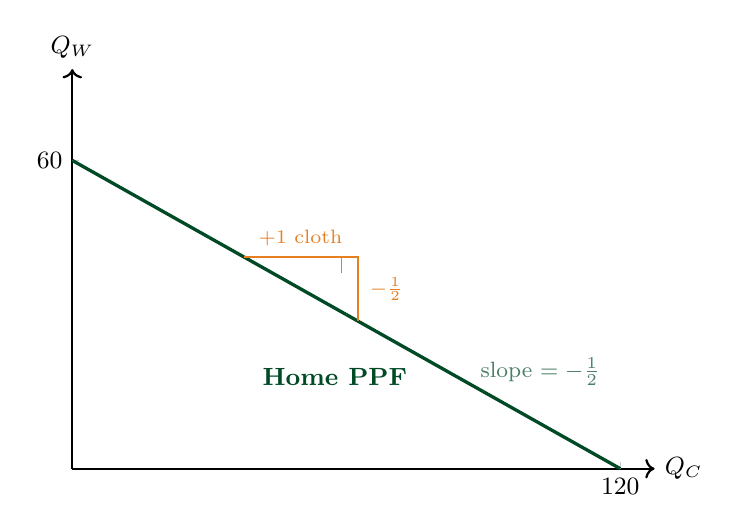
\begin{tikzpicture}[scale=1.45]

  %------------------------------------------------
  % Overlay 1: Axes
  %------------------------------------------------
  \draw[->,thick](0,0)--(5.1,0)
       node[right,font=\small]{$Q_C$};

  \draw[->,thick](0,0)--(0,3.5)
       node[above,font=\small]{$Q_W$};

  % Axis labels
  \node[left,font=\small]  at (0,2.7){60};
  \node[below,font=\small] at (4.8,0){120};

  \draw[thin,gray!40](0,2.7)--(.06,2.7);
  \draw[thin,gray!40](4.8,0)--(4.8,.06);


  %------------------------------------------------
  % Overlay 2: Start drawing the PPF
  %------------------------------------------------
  \uncover<2->{
    \draw[UNBCDark,very thick]
       (0,2.7)--(1.2,2.025);
  }


  %------------------------------------------------
  % Overlay 3: Continue drawing the PPF
  %------------------------------------------------
  \uncover<3->{
    \draw[UNBCDark,very thick]
       (1.2,2.025)--(2.4,1.35);
  }


  %------------------------------------------------
  % Overlay 4: Continue drawing the PPF
  %------------------------------------------------
  \uncover<4->{
    \draw[UNBCDark,very thick]
       (2.4,1.35)--(3.6,.675);
  }


  %------------------------------------------------
  % Overlay 5: Complete the PPF
  %------------------------------------------------
  \uncover<5->{
    \draw[UNBCDark,very thick]
       (3.6,.675)--(4.8,0);

    \node[UNBCDark,font=\small\bfseries]
       at (2.3,.8){Home PPF};
  }


  %------------------------------------------------
  % Overlay 6: Slope triangle
  %------------------------------------------------
  \uncover<6->{

    \draw[AccentOrange,thick]
       (1.5,1.855)--(2.5,1.855)--(2.5,1.292);

    % Right-angle mark
    \draw[AccentOrange,thin]
       (2.5,1.855)--(2.36,1.855)
       --(2.36,1.855-0.14);

    % Horizontal change
    \node[AccentOrange,font=\scriptsize,above]
       at (2.0,1.87)
       {$+1$ cloth};

    % Vertical change
    \node[AccentOrange,font=\scriptsize,right]
       at (2.52,1.57)
       {$-\tfrac{1}{2}$};
  }


  %------------------------------------------------
  % Overlay 7: Slope label
  %------------------------------------------------
  \uncover<7->{
    \node[
       font=\footnotesize,
       text=UNBCDark!70
    ] at (4.1,0.85)
       {slope $=-\tfrac{1}{2}$};
  }

\end{tikzpicture}
\end{column}
\end{columns}
\end{frame}

%% ─────────────────────────────────────────────────────────────
%% 12. FOREIGN PPF
%% ─────────────────────────────────────────────────────────────
\begin{frame}[shrink=15]{Foreign's Production Possibility Frontier}
\begin{columns}[T]
\begin{column}{0.46\textwidth}
\textbf{Labour constraint:}
\[a_{LC}^{*}\,Q_C^{*}+a_{LW}^{*}\,Q_W^{*}=L^{*}\]
With $a_{LC}^{*}=6$, $a_{LW}^{*}=3$, $L^{*}=120$:
\[6\,Q_C^{*}+3\,Q_W^{*}=120\]
\textbf{PPF intercepts:}
\begin{itemize}\small
  \item All cloth: $Q_C^{*\max}=20$
  \item All wine: $Q_W^{*\max}=40$
\end{itemize}
\textbf{Slope}: $-a_{LC}^{*}/a_{LW}^{*}=-2$\\[0.2em]
\emph{Steeper} than Home ($-1/2$).\\[0.3em]
\textbf{Autarky price:} $(P_C/P_W)^{*}=2$\\[0.2em]
Foreign's cloth is more expensive (higher OC) --
this gap with Home's price of $1/2$ \textbf{drives trade}.
\end{column}
\begin{column}{0.51\textwidth}

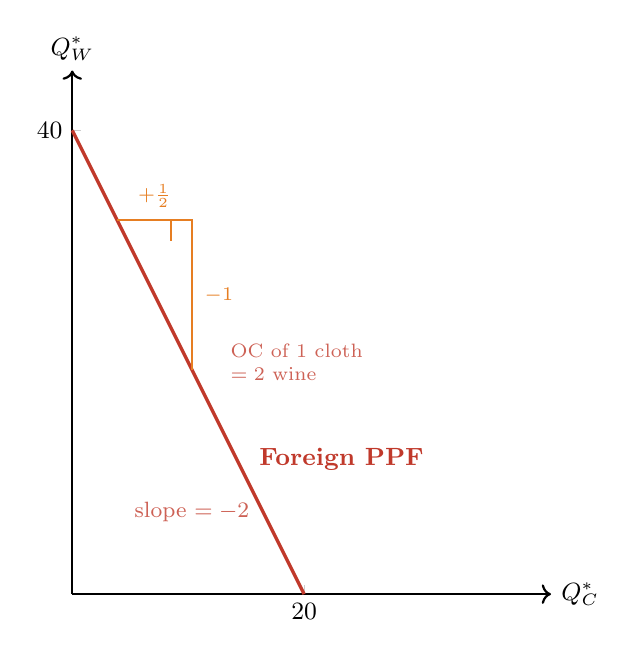
\begin{tikzpicture}[scale=1.9]

    % ------------------------------------------------
    % 1. Axes
    % ------------------------------------------------
    \uncover<1->{
        \draw[->,thick](0,0)--(3.2,0)
            node[right,font=\small]{$Q_C^{*}$};

        \draw[->,thick](0,0)--(0,3.5)
            node[above,font=\small]{$Q_W^{*}$};

        % Axis labels
        \node[left,font=\small] at (0,3.1){40};
        \node[below,font=\small] at (1.55,0){20};

        \draw[thin,gray!40](0,3.1)--(.06,3.1);
        \draw[thin,gray!40](1.55,0)--(1.55,.06);
    }

    % ------------------------------------------------
    % 2. Foreign PPF
    % ------------------------------------------------
    \uncover<2->{
        % PPF: (0,3.1) -> (1.55,0), slope = -2
        \draw[AccentRed,very thick]
            (0,3.1)--(1.55,0);

        \node[AccentRed,font=\small\bfseries]
            at (1.8,.9) {Foreign PPF};
    }

    % ------------------------------------------------
    % 3. Slope triangle
    % ------------------------------------------------
    \uncover<3->{
        \draw[AccentOrange,thick]
            (0.3,2.5)--(0.8,2.5)--(0.8,1.5);

        % Small right-angle marker
        \draw[AccentOrange,thin]
            (0.8,2.5)--(0.66,2.5)
            --(0.66,2.36);
    }

    % ------------------------------------------------
    % 4. Change in Q_C = +1/2
    % ------------------------------------------------
    \uncover<4->{
        \node[AccentOrange,font=\scriptsize,above]
            at (0.55,2.52)
            {$+\tfrac{1}{2}$};
    }

    % ------------------------------------------------
    % 5. Change in Q_W = -1
    % ------------------------------------------------
    \uncover<5->{
        \node[AccentOrange,font=\scriptsize,right]
            at (0.82,2.0)
            {$-1$};
    }

    % ------------------------------------------------
    % 6. Slope calculation
    % ------------------------------------------------
    \uncover<6->{
        \node[font=\footnotesize,text=AccentRed!80]
            at (0.8,0.55)
            {slope $=-2$};
    }

    % ------------------------------------------------
    % 7. Opportunity cost
    % ------------------------------------------------
    \uncover<7->{
        \node[
            font=\scriptsize,
            align=left,
            text=AccentRed!80
        ]
            at (1.5,1.55)
            {OC of 1 cloth\\$=2$ wine};
    }

\end{tikzpicture}

\end{column}
\end{columns}
\end{frame}













%% ─────────────────────────────────────────────────────────────
%% 13. COMPARING THE TWO COUNTRIES
%% ─────────────────────────────────────────────────────────────
\begin{frame}{Comparing Home and Foreign: The Price Gap}
\begin{center}
\begin{adjustbox}{max width=0.88\textwidth}
\begin{tabular}{lcccc}
\toprule
\textbf{Country}&$a_{LC}$&$a_{LW}$&
\textbf{Autarky $P_C/P_W$}&\textbf{CA in}\\
\midrule
Home   & 1 & 2 & $\tfrac{1}{2}$ & Cloth\\
Foreign& 6 & 3 & $2$            & Wine\\
\bottomrule
\end{tabular}
\end{adjustbox}
\end{center}
\vspace{0.3em}
\begin{columns}[T]
\begin{column}{0.53\textwidth}
\textbf{How the price gap creates trade:}
\begin{enumerate}\small
  \item Cloth is \emph{relatively cheap} in Home
        ($P_C/P_W=1/2$); wine is cheap in Foreign
        ($P_C/P_W=2$).
  \item Opening trade lets each country buy the
        relatively cheap good from the other.
  \item Any world price $p^{*}$ with $1/2 < p^{*} < 2$
        makes \textbf{both} countries better off.
\end{enumerate}
\end{column}
\begin{column}{0.44\textwidth}
\begin{insight}{The No-Trade Trap}
\small Without trade, each country is confined to its
own PPF.\\[0.2em]
The autarky price gap ($1/2$ vs.\ $2$) is a
\emph{mutually beneficial} trade opportunity: Home
can sell cloth at a price above its OC; Foreign can
sell wine at a price above its OC.
\end{insight}
\end{column}
\end{columns}
\end{frame}

%% ─────────────────────────────────────────────────────────────
%% 14. TRADE THEOREM
%% ─────────────────────────────────────────────────────────────
\begin{frame}{The Ricardian Trade Theorem}
\begin{block}{Ricardian Trade Theorem}
Under free trade with world relative price
$p^{*}\equiv P_C/P_W$, each country
\textbf{completely specialises} in its CA good
provided:
\[\frac{a_{LC}}{a_{LW}}<p^{*}<\frac{a_{LC}^{*}}{a_{LW}^{*}}
  \quad\Longleftrightarrow\quad \tfrac{1}{2}<p^{*}<2\]
\end{block}
\vspace{0.3em}
\begin{columns}[T]
\begin{column}{0.53\textwidth}
\textbf{Intuition:}
\begin{itemize}\small
  \item $p^{*}>1/2$: Home earns more per hour in cloth
        $\Rightarrow$ all labour to cloth.
  \item $p^{*}<2$: Foreign earns more per hour in wine
        $\Rightarrow$ Foreign fully in wine.
  \item \textbf{Home exports cloth; Foreign exports wine.}
\end{itemize}
\end{column}
\begin{column}{0.44\textwidth}
\begin{varbox}
\small\textbf{Edge cases:}\\[0.2em]
$p^{*}=1/2$: Home indifferent (kink of RS).\\
$p^{*}=2$: Foreign indifferent.\\[0.2em]
$p^{*}$ outside $(1/2,\,2)$: one country does not
specialise completely; equilibrium is at a vertical
segment of the RS curve.
\end{varbox}
\end{column}
\end{columns}
\end{frame}

%% ═══════════════════════════════════════════════════════════
%%  PART 3 — WORLD EQUILIBRIUM AND GAINS
%% ═══════════════════════════════════════════════════════════

%% ─────────────────────────────────────────────────────────────
%% 15. WORLD RELATIVE SUPPLY
%% ─────────────────────────────────────────────────────────────
\begin{frame}{World Relative Supply and Demand}
\begin{columns}[T]
\begin{column}{0.53\textwidth}
\textbf{World Relative Supply (RS)} = world cloth
output $\div$ world wine output, as a function of $p$.
\begin{itemize}\small
  \item $p<1/2$: both prefer wine $\Rightarrow$ RS $=0$.
  \item $p=1/2$: Home indifferent.
  \item $1/2<p<2$: both specialise.
        
  \item $p=2$: Foreign indifferent; RS $\to\infty$.
\end{itemize}
\textbf{World Relative Demand (RD)}: downward-sloping.
Higher $p$ $\Rightarrow$ shift toward wine.\\[0.3em]
\textbf{Equilibrium} $p^{*}$: where RD crosses RS.
If RD crosses the \emph{inelastic segment}, both countries
completely specialise.
\end{column}
\begin{column}{0.44\textwidth}
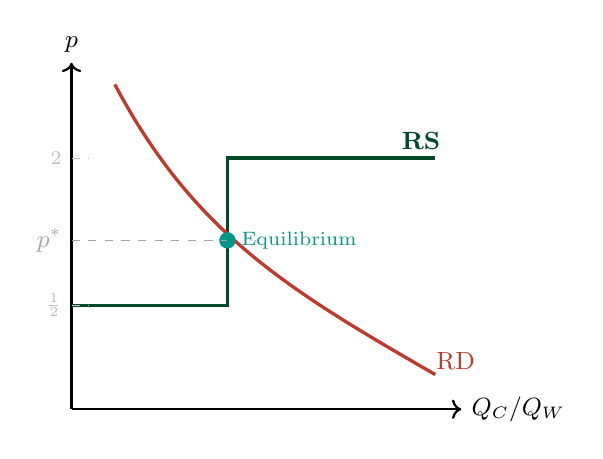
\begin{tikzpicture}[scale=1.1]

    %------------------------------------------------
    % Axes
    %------------------------------------------------
    \draw[->,thick]
        (0,0)--(4.5,0)
        node[right,font=\small]{$Q_C/Q_W$};

    \draw[->,thick]
        (0,0)--(0,4.0)
        node[above,font=\small]{$p$};

    %------------------------------------------------
    % RS: Step function
    %------------------------------------------------
    \uncover<1->{
        \draw[UNBCDark,very thick]
            (0,1.2)--(1.8,1.2)
            --(1.8,2.9)--(4.2,2.9);

        \node[
            UNBCDark,
            font=\small\bfseries,
            right
        ] at (3.7,3.1){RS};
    }

    %------------------------------------------------
    % RD
    %------------------------------------------------
    \uncover<2->{
        \draw[AccentRed,very thick]
            (0.5,3.75)
            to[out=-62,in=150]
            (4.2,0.4);

        \node[
            AccentRed,
            font=\small,
            right
        ] at (4.1,0.56){RD};
    }

    %------------------------------------------------
    % Equilibrium
    %------------------------------------------------
    \uncover<3->{
        \filldraw[
            AccentTeal
        ] (1.8,1.95) circle(2.5pt);

        \draw[dashed,gray!70]
            (0,1.95)
            node[left,font=\small]{$p^{*}$}
            --(1.8,1.95);

        \node[
            AccentTeal,
            font=\scriptsize,
            right
        ] at (1.85,1.95){Equilibrium};
    }

    %------------------------------------------------
    % Price references
    %------------------------------------------------
    \uncover<4->{
        \draw[dashed,gray!50]
            (0,1.2)
            node[left,font=\scriptsize]{$\tfrac{1}{2}$}
            --(0.2,1.2);

        \draw[dashed,gray!50]
            (0,2.9)
            node[left,font=\scriptsize]{$2$}
            --(0.2,2.9);
    }

\end{tikzpicture}
\end{column}
\end{columns}
\end{frame}

%% ─────────────────────────────────────────────────────────────
%% 16. GAINS FROM TRADE: HOME
%% ─────────────────────────────────────────────────────────────
\begin{frame}{Gains from Trade: Home}
\begin{columns}[T]
\begin{column}{0.45\textwidth}
\textbf{Autarky}: Home consumes on PPF
(slope $-1/2$).\\[0.4em]
\textbf{Free trade at $p^{*}=1$:}
\begin{enumerate}\small
  \item Specialise fully in cloth: produce 120 cloth,
        0 wine.
  \item Sell cloth, buy wine at $p^{*}=1$.
  \item Budget line (trade line) through production
        point $(120,0)$ with slope $-1$.
  \item Home reaches a higher indifference curve
        \textbf{above} the PPF.
\end{enumerate}
\vspace{0.2em}
\textbf{The gain:} domestic cost of wine $= 2$
cloth/wine; trade cost $= 1$ cloth/wine.
Trade saves 1 unit of cloth per wine imported.
\end{column}
\begin{column}{0.52\textwidth}
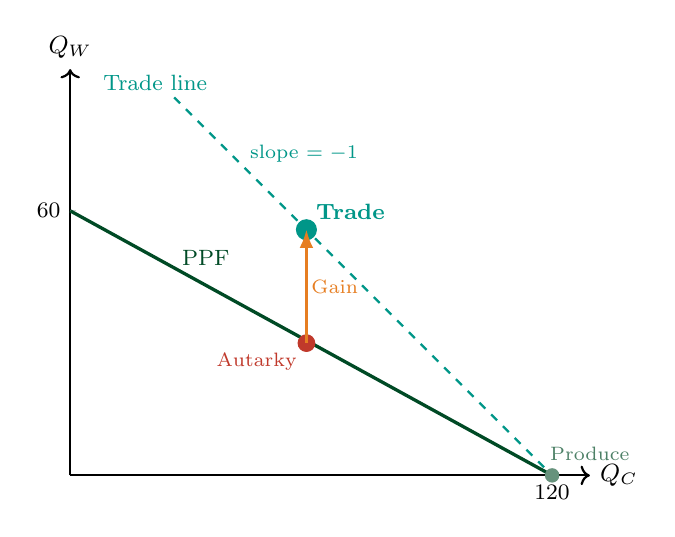
\begin{tikzpicture}[scale=1.2]

  %------------------------------------------------
  % Axes
  %------------------------------------------------
  \draw[->,thick](0,0)--(5.5,0)
      node[right,font=\small]{$Q_C$};

  \draw[->,thick](0,0)--(0,4.3)
      node[above,font=\small]{$Q_W$};

  \node[left,font=\footnotesize] at (0,2.8){60};
  \node[below,font=\footnotesize] at (5.1,0){120};

  \draw[thin,gray!40](0,2.8)--(.06,2.8);
  \draw[thin,gray!40](5.1,0)--(5.1,.06);

  %------------------------------------------------
  % Home PPF
  % Always visible
  %------------------------------------------------
  \draw[UNBCDark,very thick]
      (0,2.8)--(5.1,0);

  \node[UNBCDark,font=\footnotesize,left]
      at (1.79,2.3){PPF};

  %------------------------------------------------
  % Overlay 2: Trade line
  %------------------------------------------------
  \uncover<2->{
    \draw[AccentTeal,thick,dashed]
        (1.1,4.0)--(5.1,0);

    \node[AccentTeal,font=\footnotesize]
        at (0.9,4.15){Trade line};

    \node[AccentTeal,font=\scriptsize,right]
        at (1.8,3.4){slope $=-1$};
  }

  %------------------------------------------------
  % Overlay 2: Production point
  %------------------------------------------------
  \uncover<2->{
    \filldraw[UNBCDark!60]
        (5.1,0) circle(2pt);

    \node[UNBCDark!70,font=\scriptsize,above]
        at (5.5,0.05){Produce};
  }

  %------------------------------------------------
  % Overlay 3: Autarky
  %------------------------------------------------
  \uncover<3->{
    \filldraw[AccentRed]
        (2.5,1.4) circle(2.5pt);

    \node[AccentRed,font=\scriptsize,below left]
        at (2.5,1.4){Autarky};
  }

  %------------------------------------------------
  % Overlay 3: Trade consumption
  %------------------------------------------------
  \uncover<3->{
    \filldraw[AccentTeal]
        (2.5,2.6) circle(3pt);

    \node[AccentTeal,font=\footnotesize,above right]
        at (2.5,2.6){\textbf{Trade}};
  }

  %------------------------------------------------
  % Overlay 4: Gain arrow
  %------------------------------------------------
  \uncover<4->{
    \draw[-{Latex[width=5pt]},AccentOrange,thick]
        (2.5,1.4)--(2.5,2.6);

    \node[AccentOrange,font=\scriptsize,right]
        at (2.45,2.0){Gain};
  }

\end{tikzpicture}
\end{column}
\end{columns}
\end{frame}

%% ─────────────────────────────────────────────────────────────
%% 17. GAINS FROM TRADE: FOREIGN
%% ─────────────────────────────────────────────────────────────
\begin{frame}{Gains from Trade: Foreign}
\begin{columns}[T]
\begin{column}{0.45\textwidth}
\textbf{Foreign autarky}: PPF slope $=-2$.\\[0.4em]
\textbf{Free trade at $p^{*}=1$:}
\begin{enumerate}\small
  \item Specialise fully in wine: produce 40 wine, 0
        cloth.
  \item Sell wine, buy cloth at $p^{*}=1$.
  \item $p^{*}=1<2$: cloth cheaper via trade than
        domestic production.
  \item Trade line slope $=-1$ (flatter than PPF
        slope $=-2$).
\end{enumerate}
\vspace{0.2em}
\textbf{The gain:} domestic cost of cloth $= 2$
wine/cloth; trade cost $= 1$ wine/cloth.
Trade halves Foreign's cost of obtaining cloth.
\end{column}
\begin{column}{0.52\textwidth}
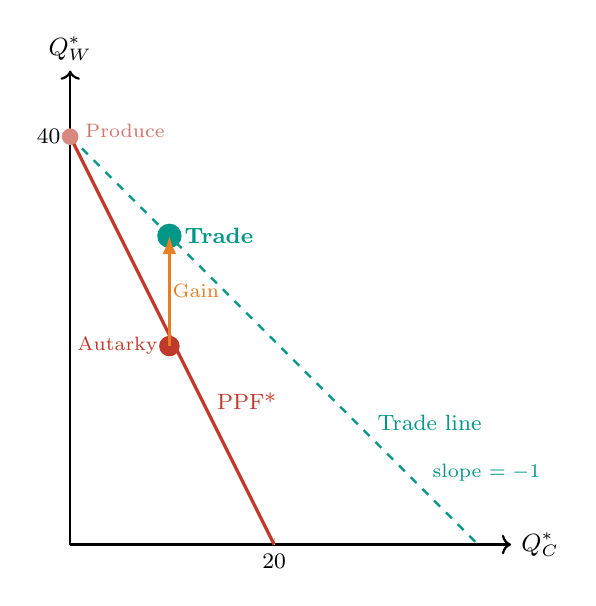
\begin{tikzpicture}[scale=1.4]

  %------------------------------------------------
  % 1. Axes and labels
  %------------------------------------------------
  \draw[->,thick]
      (0,0)--(4.0,0)
      node[right,font=\small]{$Q_C^{*}$};

  \draw[->,thick]
      (0,0)--(0,4.3)
      node[above,font=\small]{$Q_W^{*}$};

  %------------------------------------------------
  % 2. Intercepts
  %------------------------------------------------
  \uncover<2->{
    \node[left,font=\footnotesize] at (0,3.7){40};
    \node[below,font=\footnotesize] at (1.85,0){20};

    \draw[thin,gray!40](0,3.7)--(.06,3.7);
    \draw[thin,gray!40](1.85,0)--(1.85,.06);
  }

  %------------------------------------------------
  % 3. Foreign PPF
  %------------------------------------------------
  \uncover<3->{
    \draw[AccentRed,very thick]
        (0,3.7)--(1.85,0);

    \node[AccentRed,font=\footnotesize]
        at (1.6,1.3){PPF*};
  }

  %------------------------------------------------
  % 4. Trade line
  %------------------------------------------------
  \uncover<4->{
    \draw[AccentTeal,thick,dashed]
        (0,3.7)--(3.7,0);

    \node[AccentTeal,font=\footnotesize,right]
        at (2.7,1.1){Trade line};

    \node[AccentTeal,font=\scriptsize,right]
        at (3.2,0.65){slope $=-1$};
  }

  %------------------------------------------------
  % 5. Production point
  %------------------------------------------------
  \uncover<5->{
    \filldraw[AccentRed!60]
        (0,3.7) circle(2pt);

    \node[AccentRed!70,font=\scriptsize,right]
        at (0.05,3.75){Produce};
  }

  %------------------------------------------------
  % 6. Autarky point
  %------------------------------------------------
  \uncover<6->{
    \filldraw[AccentRed]
        (0.9,1.8) circle(2.5pt);

    \node[AccentRed,font=\scriptsize,left]
        at (0.88,1.8){Autarky};
  }

  %------------------------------------------------
  % 7. Trade point
  %------------------------------------------------
  \uncover<7->{
    \filldraw[AccentTeal]
        (0.9,2.8) circle(3pt);

    \node[AccentTeal,font=\footnotesize,right]
        at (0.95,2.8){\textbf{Trade}};
  }

  %------------------------------------------------
  % 8. Gain from trade
  %------------------------------------------------
  \uncover<8->{
    \draw[-{Latex[width=5pt]},AccentOrange,thick]
        (0.9,1.8)--(0.9,2.8);

    \node[AccentOrange,font=\scriptsize,right]
        at (0.84,2.3){Gain};
  }

\end{tikzpicture}
\end{column}
\end{columns}
\end{frame}

%% ─────────────────────────────────────────────────────────────
%% 18. TERMS OF TRADE
%% ─────────────────────────────────────────────────────────────
\begin{frame}{The Terms of Trade: Definition and Welfare}
\begin{columns}[T]
\begin{column}{0.53\textwidth}
\begin{block}{Terms of Trade (ToT)}
\small\textbf{ToT for Home} $=$ export price $\div$
import price $= P_C/P_W = p^{*}$.\\[0.2em]
Mutual gain requires:
$\;\dfrac{a_{LC}}{a_{LW}}<p^{*}<\dfrac{a_{LC}^{*}}{a_{LW}^{*}}$
\end{block}
\vspace{0.3em}
\textbf{Effect of ToT on welfare:}
\begin{itemize}\small
  \item \textbf{Higher $p^{*}$ (toward 2):} Home gains
        more; each cloth exported buys more wine.
  \item \textbf{Lower $p^{*}$ (toward $1/2$):} Foreign
        gains more.
  \item Both \emph{always} gain relative to autarky
        as long as $1/2 < p^{*} < 2$.
\end{itemize}
\textbf{Equilibrium $p^{*}$:} RS $=$ RD.
\end{column}
\begin{column}{0.44\textwidth}
\begin{canadex}[Canada's Terms of Trade]
\footnotesize Canada exports energy, agriculture,
aircraft; imports manufactures, electronics.\\[0.3em]
\textbf{2002--2014}: Rising oil prices raised Canada's
ToT sharply.  Real national income rose ${\approx}15\%$
more than real GDP~-- a pure ToT gain.\\[0.3em]
\textbf{After 2014}: Oil price collapse worsened ToT.
Alberta entered recession; Bank of Canada cut rates
in 2015--16.\\[0.2em]
Ricardian lesson: exporters of a rising-price good gain.
\end{canadex}
\end{column}
\end{columns}
\end{frame}

%% ═══════════════════════════════════════════════════════════
%%  PART 4 — WAGES AND EMPIRICS
%% ═══════════════════════════════════════════════════════════

%% ─────────────────────────────────────────────────────────────
%% 19. WAGES UNDER TRADE
%% ─────────────────────────────────────────────────────────────
\begin{frame}[shrink=15]{Wages, Productivity, and Trade}
\begin{columns}[T]
\begin{column}{0.54\textwidth}
\textbf{Home's wage} (specialises in cloth):
\[w=\frac{P_C}{a_{LC}}=\frac{p^{*}P_W}{a_{LC}},
  \qquad w^{*}=\frac{P_W}{a_{LW}^{*}}\]
\textbf{Relative wage ratio:}
\[\frac{w}{w^{*}}=p^{*}\!\cdot\!\frac{a_{LW}^{*}}{a_{LC}}\]
With $p^{*}=1$, $a_{LC}=1$, $a_{LW}^{*}=3$:
$\;w/w^{*}=3$.\\[0.3em]
Home earns $3\times$ Foreign wages~-- because it is
$3$--$6\times$ more productive.\\[0.3em]
\textbf{Unit labour costs:}
\begin{itemize}\small
  \item Cloth: Home $=3w^{*}$; Foreign $=6w^{*}$.
        Home cheaper. \checkmark
  \item Wine: Home $=6w^{*}$; Foreign $=3w^{*}$.
        Foreign cheaper. \checkmark
\end{itemize}
\end{column}
\begin{column}{0.43\textwidth}
\begin{insight}{Wage Result}
\small Higher productivity $\Rightarrow$ higher wages.\\
But high wages do \emph{not} prevent trade.\\[0.3em]
Home's wage advantage is exactly offset by its
productivity advantage in cloth.\\[0.3em]
Each country is competitive in its CA sector
\emph{regardless} of the absolute wage level.
\end{insight}
\vspace{0.3em}
\begin{varbox}
\footnotesize\textbf{Relative-wage bounds:}
\[\frac{a_{LC}^{*}}{a_{LC}}>\frac{w}{w^{*}}
  >\frac{a_{LW}^{*}}{a_{LW}}\]
In example: $6>w/w^{*}>3/2$.\\
At $p^{*}=1$: $w/w^{*}=3$ (\checkmark inside bounds).
\end{varbox}
\end{column}
\end{columns}
\end{frame}

%% ─────────────────────────────────────────────────────────────
%% 20. PRODUCTIVITY DATA
%% ─────────────────────────────────────────────────────────────
\begin{frame}{Do Wages Reflect Productivity? The Ricardian Prediction}
\begin{columns}[T]
\begin{column}{0.53\textwidth}
\textbf{Ricardian model predicts:} $w\propto$ labour
productivity.
\vspace{0.3em}
\begin{adjustbox}{max width=\columnwidth}
\begin{tabular}{lrrr}
\toprule
\textbf{Country} & \textbf{Wage} &
\textbf{Productivity} & \textbf{Unit}\\
 & (USD/hr) & (USA\,=\,100) & \textbf{labour cost}\\
\midrule
USA         & 35.0 & 100 & 35.0\textcent/unit\\
Germany     & 43.0 & 108 & 39.8\textcent/unit\\
South Korea & 22.0 &  67 & 32.8\textcent/unit\\
Mexico      &  5.0 &  28 & 17.9\textcent/unit\\
Bangladesh  &  0.6 &   4 & 15.0\textcent/unit\\
\bottomrule
\multicolumn{4}{l}{\tiny BLS, ILO, World Bank (2019)}
\end{tabular}
\end{adjustbox}
\end{column}
\begin{column}{0.44\textwidth}
\textbf{Key findings:}
\begin{itemize}\small
  \item High-productivity countries have high wages:
        Ricardian prediction \textbf{confirmed}.
  \item Unit labour cost varies less than wages~--
        productivity differences offset wage differences.
  \item Bangladesh's low wages reflect low productivity,
        not a threat to Canadian workers in
        high-productivity sectors.
\end{itemize}
\vspace{0.3em}
\begin{insight}{Verdict}
\footnotesize Trade with low-wage countries does
\emph{not} impoverish high-wage countries~-- because
low wages come with low productivity.
\end{insight}
\end{column}
\end{columns}
\end{frame}

%% ─────────────────────────────────────────────────────────────
%% 22. BANGLADESH vs CHINA
%% ─────────────────────────────────────────────────────────────
\begin{frame}{Bangladesh vs.\ China: CA in Action}
\begin{columns}[T]
\begin{column}{0.53\textwidth}
\textbf{Both export garments.  How?}
\begin{itemize}\small
  \item China has higher absolute productivity in
        \emph{both} garments and electronics.
  \item But China's \textbf{OC of garments is rising}:
        its CA shifts toward electronics, AI, and
        capital-intensive goods.
  \item Bangladesh's OC of garments remains low~--
        it lacks a competitive electronics sector.
  \item China moves up the value chain; Bangladesh stays
        in garments.
\end{itemize}
\vspace{0.2em}
\begin{insight}{Confirmed}
\footnotesize Each country exports where its
\emph{relative} cost is lowest, not where its absolute
cost is lowest.
\end{insight}
\end{column}
\begin{column}{0.44\textwidth}
\begin{adjustbox}{max width=\columnwidth}
\begin{tabular}{lrr}
\toprule
 & \textbf{Bangladesh} & \textbf{China}\\
\midrule
Mfg wage (USD/hr) & 0.57 & 4.99\\
Garment exports   & \$34B & \$185B\\
Electronics exp.  & \$0.4B & \$842B\\
\midrule
Garments/Elect.   & \textbf{85}$\times$ &
                    \textbf{0.2}$\times$\\
\bottomrule
\multicolumn{3}{l}{\tiny ITC, World Bank (2019)}
\end{tabular}
\end{adjustbox}
\vspace{0.3em}

\end{column}
\end{columns}
\end{frame}


%% ─────────────────────────────────────────────────────────────
%% 25. WORKED EXAMPLE SETUP (Quiz 1)
%% ─────────────────────────────────────────────────────────────
\begin{frame}{Worked Example: Wine and Cheese}
\begin{worked}
Two countries, \textbf{Home} and \textbf{Foreign}; two
goods, \textbf{Wine (W)} and \textbf{Cheese (C)}.
$L=L^{*}=120$ hours of labour each.
\end{worked}
\vspace{0.3em}
\begin{center}
\begin{adjustbox}{max width=0.60\textwidth}
\begin{tabular}{lcc}
\toprule
 & Wine (hr/unit) & Cheese (hr/unit)\\
\midrule
Home    & $a_{LW}=2$     & $a_{LC}=1$  \\
Foreign & $a_{LW}^{*}=6$ & $a_{LC}^{*}=2$\\
\bottomrule
\end{tabular}
\end{adjustbox}
\end{center}
\vspace{0.3em}
\begin{columns}[T]
\begin{column}{0.48\textwidth}
\textbf{Questions:}
\begin{enumerate}[(a)]\small
  \item Max Wine and Cheese for each country.
  \item OC of Wine in terms of Cheese (each country).
  \item Which country has CA in Wine?  In Cheese?
  \item At $P_W/P_C=2.5$: who exports what?
\end{enumerate}
\end{column}
\begin{column}{0.49\textwidth}
\textbf{Steps:}
\begin{enumerate}\small
  \item Max Q $= L/a_L$.
  \item OC of Wine $= a_{LW}/a_{LC}$.
  \item Lower OC $\Rightarrow$ CA in Wine.
  \item Compare $p^{*}$ to autarky price:\\
        $p^{*}>$ autarky $\Rightarrow$ export Wine.
\end{enumerate}
\end{column}
\end{columns}
\end{frame}

%% ─────────────────────────────────────────────────────────────
%% 26. WORKED EXAMPLE SOLUTION
%% ─────────────────────────────────────────────────────────────
\begin{frame}{Worked Example: Solution}
\begin{columns}[T]
\begin{column}{0.53\textwidth}
\textbf{(a) Max production} ($L=120$):
\begin{itemize}\small
  \item Home: $Q_W^{\max}=60$; $Q_C^{\max}=120$.
  \item Foreign: $Q_W^{*\max}=20$; $Q_C^{*\max}=60$.
\end{itemize}
\textbf{(b) OC of Wine:}
\begin{itemize}\small
  \item Home: $a_{LW}/a_{LC}=2/1=\mathbf{2}$ Cheese.
  \item Foreign: $6/2=\mathbf{3}$ Cheese.
\end{itemize}
\textbf{(c) CA:}\; $2<3$
$\Rightarrow$ \textbf{Home: Wine};\;
\textbf{Foreign: Cheese}.\\[0.3em]
\textbf{(d) At $P_W/P_C=2.5$:}
\begin{itemize}\small
  \item Home autarky price $=2<2.5$: Wine is profitable.
        $\Rightarrow$ \textbf{Home exports Wine}.
  \item Foreign autarky price $=3>2.5$: Wine cheaper
        via trade.
        $\Rightarrow$ \textbf{Foreign exports Cheese}.
\end{itemize}
\end{column}
\begin{column}{0.44\textwidth}
\begin{insight}{Key Check}
\footnotesize Valid range for $P_W/P_C$: $(2,\;3)$.\\
$p^{*}=2.5$ lies in this range. \checkmark\\[0.3em]
$2<2.5$: Home exports Wine. \checkmark\\
$3>2.5$: Foreign exports Cheese. \checkmark\\[0.3em]
Both specialise completely; both gain.
\end{insight}
\vspace{0.4em}
\begin{varbox}
\footnotesize\textbf{Mutual-gain check:}\\[0.1em]
Home gains if $p^{*}>2$. \checkmark\\
Foreign gains if $p^{*}<3$. \checkmark\\
$p^{*}=2.5$ satisfies both. \checkmark
\end{varbox}
\end{column}
\end{columns}
\end{frame}


%% ─────────────────────────────────────────────────────────────
%% 28. LIMITATIONS
%% ─────────────────────────────────────────────────────────────
\begin{frame}[shrink=5]{Limitations and What Comes Next}
\begin{columns}[T]
\begin{column}{0.52\textwidth}
\textbf{What the Ricardian model does well:}
\begin{itemize}\small
  \item Explains the \emph{direction} of trade (CA).
  \item Shows \emph{mutual gains} for all countries.
  \item Connects productivity to wages (empirically
        supported).
  \item Refutes the pauper-labour fallacy.
  \item Generates testable predictions (MacDougall).
\end{itemize}
\vspace{0.3em}
\textbf{What it misses:}
\begin{itemize}\small
  \item Complete specialisation (never fully observed).
  \item No capital or land (factor endowments ignored).
  \item No losers within a country.
  \item No economies of scale; no intra-industry trade.
\end{itemize}
\end{column}
\begin{column}{0.45\textwidth}
\begin{insight}{Building Up the Model}
\begin{itemize}\small
  \item \textbf{Ch.~4} (Specific Factors): Add capital
        and land.  Trade creates winners and losers
        \emph{within} a country.
  \item \textbf{Ch.~5} (H-O): Long run~-- both factors
        mobile.  Factor endowments determine CA.
  \item \textbf{Ch.~7} (EoS): Increasing returns
        explain intra-industry trade.
\end{itemize}
\end{insight}
\vspace{0.3em}
\begin{varbox}
\small\textbf{Ricardian $\subset$ Specific Factors
$\subset$ H-O}\\[0.1em]
Each model is a special case of the next.
\end{varbox}
\end{column}
\end{columns}
\end{frame}

%% ─────────────────────────────────────────────────────────────
%% 29. KEY POINTS
%% ─────────────────────────────────────────────────────────────
\begin{frame}{Key Points}
\begin{columns}[T]
\begin{column}{0.57\textwidth}
\begin{enumerate}\small
  \item \textbf{Comparative advantage}, not absolute
        advantage, determines trade.  Export where OC
        is \emph{lowest}.
  \item OC $=$ ratio of ULRs: $a_{LC}/a_{LW}$.
  \item \textbf{Ricardian PPF is linear} (constant OC);
        slope $= -a_{LC}/a_{LW} =$ autarky price.
  \item Free trade $\Rightarrow$
        \textbf{complete specialisation} in CA good.
  \item Both countries \textbf{consume beyond PPFs}~--
        mutual gains.
  \item \textbf{ToT} must lie strictly between the two
        autarky prices.
  \item \textbf{Wages track productivity}: high wages
        reflect high productivity; all countries gain.
  \item \textbf{Pauper-labour fallacy} is wrong:
        unit labour cost, not wages alone, matters.
\end{enumerate}
\end{column}
\begin{column}{0.40\textwidth}
\begin{block}{Next Lecture: Chapter 4}
\textbf{Specific Factors and Income Distribution}\\[0.3em]
\small What happens in the short run when capital is
locked into specific sectors?\\[0.2em]
Who wins and who loses from trade when factor mobility
is limited?\\[0.2em]
Why do some workers and firms lobby against free trade
even when the nation gains?
\end{block}
\end{column}
\end{columns}
\end{frame}

%% ─────────────────────────────────────────────────────────────
%% 30. Refereces
%% ─────────────────────────────────────────────────────────────
\begin{frame}{Key Readings}




\begin{itemize}\footnotesize
  \item Ricardo, D.\ (1817),
        \textit{Principles of Political Economy},
        Ch.~7.
  \item MacDougall (1951), ``British and American
        Exports,'' \textit{Economic Journal}.
  \item Balassa (1963),
        \textit{Review of Economics and Statistics}.
  \item Golub \& Hsieh (2000),
        \textit{Review of International Economics}.
\end{itemize}


\end{frame}

\end{document}
